\documentclass{ws-ijprai}

\usepackage{pdfpages}
\usepackage{xcolor}
\usepackage{lipsum}
\usepackage[letterpaper, margin=1in]{geometry}
\usepackage{algorithm, algpseudocode}
\usepackage{graphicx}
\usepackage{float}
\usepackage{hyperref}
\usepackage[margin=1in,font=small]{caption}
\usepackage{subfig}

\newcommand{\subheader}[1]{\bigskip\begin{center}\textbf{#1}\end{center}}
\newcommand{\subsubheader}[1]{\smallskip\begin{center}\textit{#1}\end{center}}
%\newcommand{\subsubheader}[1]{\begin{center}\textit{#1}\end{center}}

\newcommand{\warn}[1]{{\color{red}#1}}

\begin{document}

\markboth{Braden Hoagland}{Kaggle Write-Up}

% =====
% TITLE
% =====
\title{\uppercase{Kaggle Competition Write-Up}}
\author{Braden Hoagland \\ Kaggle username: bradenhoagland}
\address{COMPSCI 671: Machine Learning}

\maketitle
\thispagestyle{empty}

% ====================
% EXPLORATORY ANALYSIS
% ====================
\subheader{Exploratory Analysis}

To begin exploring the training data, I created density plots for the values of each feature. Figure \ref{fig:densities} shows two of these plots.

\begin{figure}[H]
  \centering
  \subfloat[id]{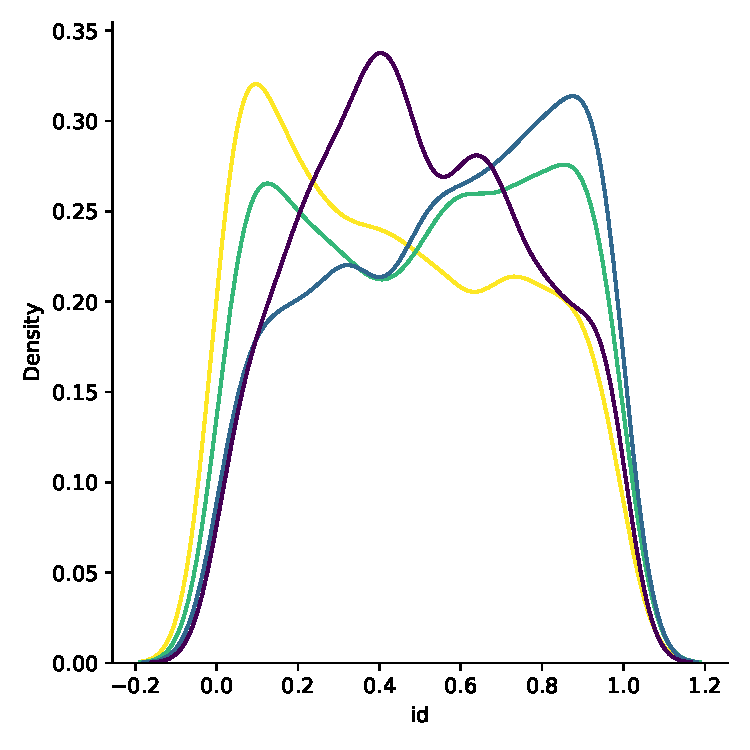
\includegraphics[width=0.4\textwidth]{img/density/id.pdf}}
  \subfloat[number of reviews]{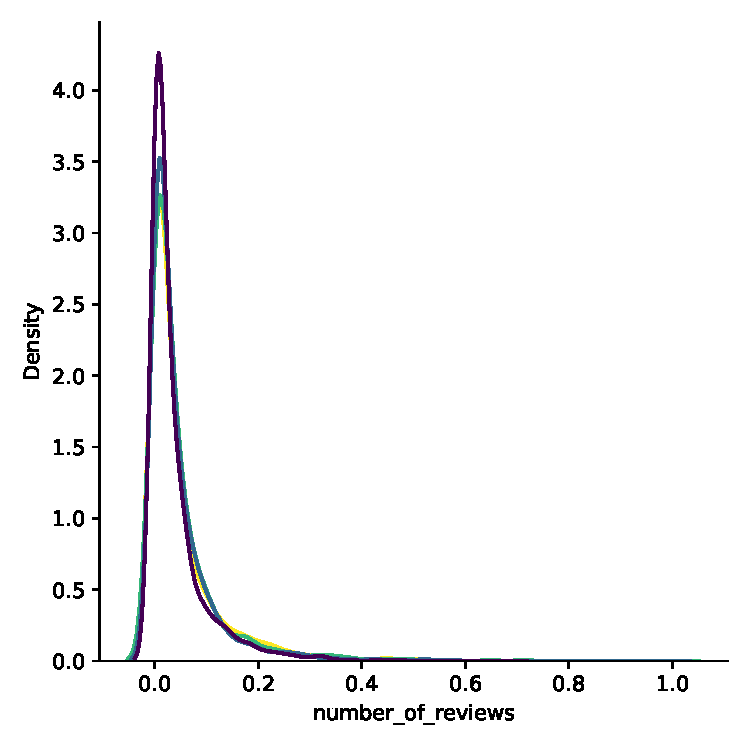
\includegraphics[width=0.4\textwidth]{img/density/number_of_reviews.pdf}}
  \caption{Density plots for two of the features. Purple lines correspond to the density of price label 1, blue for price 2, green for price 3, and yellow for price 4.}
  \label{fig:densities}
\end{figure}

After making the density plots, it was obvious that the `id' feature was random. I also noticed that the `is\_business\_travel\_ready' had only one value. As a result, I removed both of them from the dataset.

Additionally, I used these density plots to experiment with setting thresholds on the data. Note that with the number\_of\_reviews feature, almost all values are less than 0.4 (note that these quantities were already normalized, thus why the number of reviews is less than 1). One way of removing outliers from the data would be to set a threshold at 0.4. If a data point's number of reviews falls above 0.4, then it is removed from the dataset. I created thresholds like this for all features that seemed to have skewed distributions.

My tests with these ``outliers" removed yielded results that were strictly worse than when I included all the datapoints, which insinuates that I was not lenient enough with my thresholds. Because of the large number of features that I would have to manually tune, I focused on other forms of data analysis instead of this method of outlier removal.

I then examined the correlation between the different features. Figure \ref{fig:corr} shows a heatmap that represents the correlation matrix, where the $x$ and $y$-axes are the same: namely, they are each composed of every (non-removed) feature. I did not include the axis ticks because of formatting issues in this document, but I was able determine which of the features had the largest correlation. These pairs are:
\begin{itemize}
	\item reviews\_per\_month and number\_of\_reviews
	\item require\_guest\_profile\_picture and require\_guest\_phone\_verification
	\item bedrooms and bathrooms and beds
	\item guests\_included and beds, and
	\item host\_is\_superhost and reviews\_per\_month.
\end{itemize}

\begin{figure}[H]
	\centering
	\subfloat{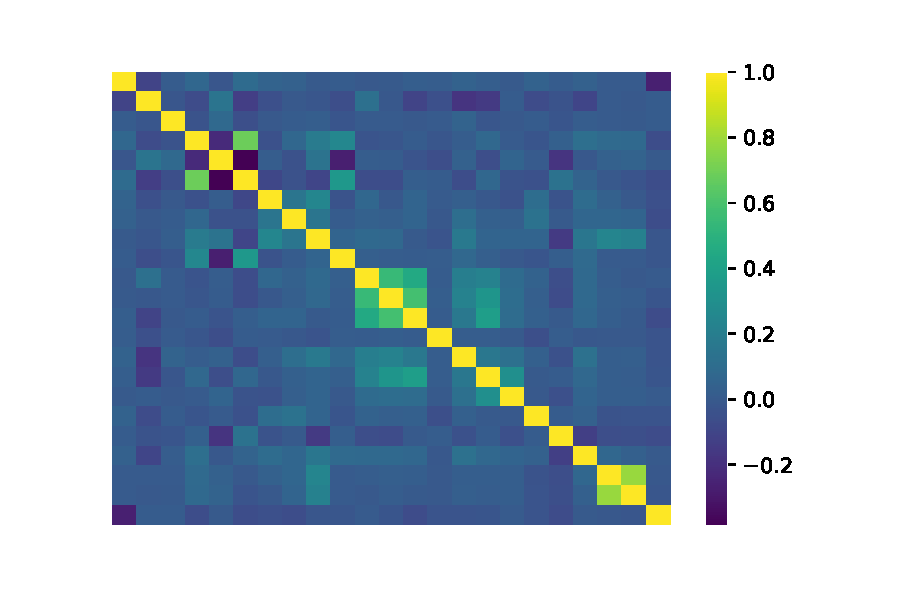
\includegraphics[width=0.4\linewidth]{img/corr/matrix.pdf}}
	\subfloat{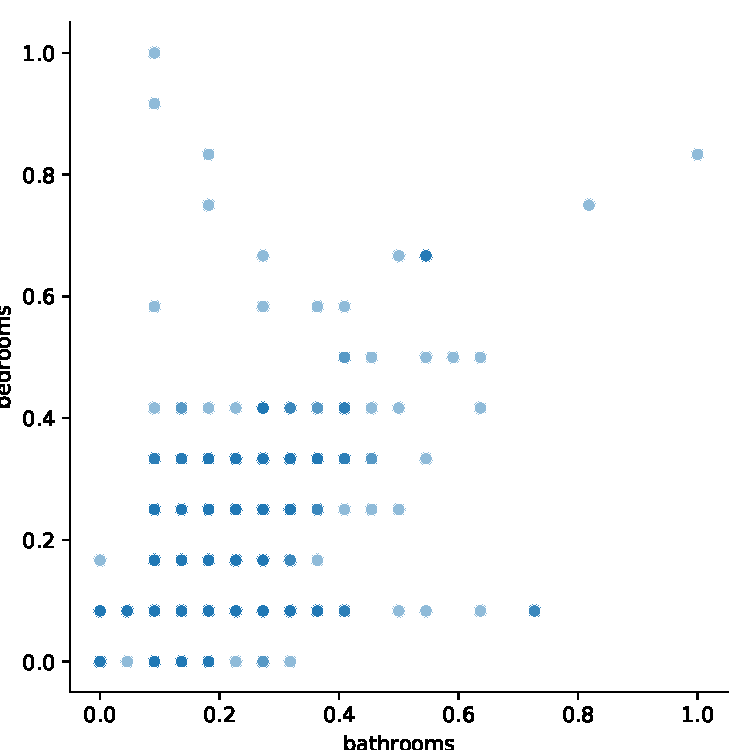
\includegraphics[width=0.3\linewidth]{img/corr/reviews.pdf}}
	\caption{The coorrelation for all remaining features, as well as an example of the correlation between bathrooms and bedrooms.}
	\label{fig:corr}
\end{figure}

I noted these correlations, and later on during training ran ablation tests with different pairs of correlated variables removed. I then kept the features that yielded the best results. I ultimately decided to remove number\_of\_reviews and require\_guest\_phone\_verification from the dataset, as these yielded the models with the best validation accuracies.

\subsubheader{Feature Engineering}

I then tried to engineer some new features for the dataset that could take into account extra domain knowledge. The first feature I tried to construct was a notion of population density in each neighborhood. I determined the longitude and latitude of each neighborhood, and planned on comparing these to population density data from Buenos Aires in order to create a new `population\_density' feature for each data point.

However, I was unable to actually find population density data for Buenos Aires, so instead I calculated the length of the geodesic between each neighborhood and the center of the city. My intuition here was that the population density should be correlated with the distance to the center of the city. This gave me a new `distance' feature that I appended to all data points and used for the remainder of my experiments.

\subsubheader{Data Clusters}

I wanted to experiment with clustering the data as a means of preprocessing, so I visually examined the data using the t-SNE and PCA algorithms. Figure \ref{fig:cluster-labels} shows the result of running both algorithms on the data to embed it into 2 dimensions.

\begin{figure}[H]
  \centering
  \subfloat[PCA]{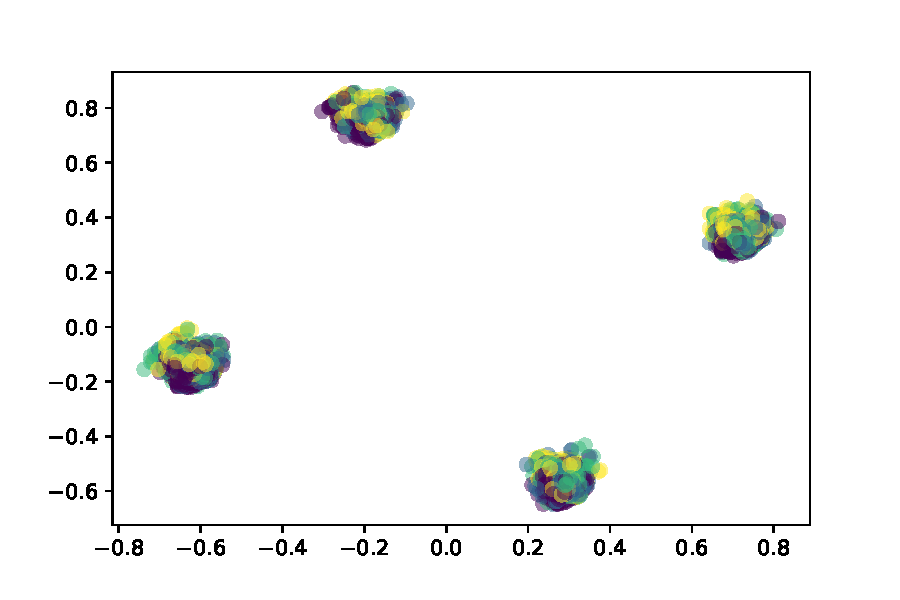
\includegraphics[width=0.4\textwidth]{img/clusters/labels.pdf}}
  \subfloat[t-SNE]{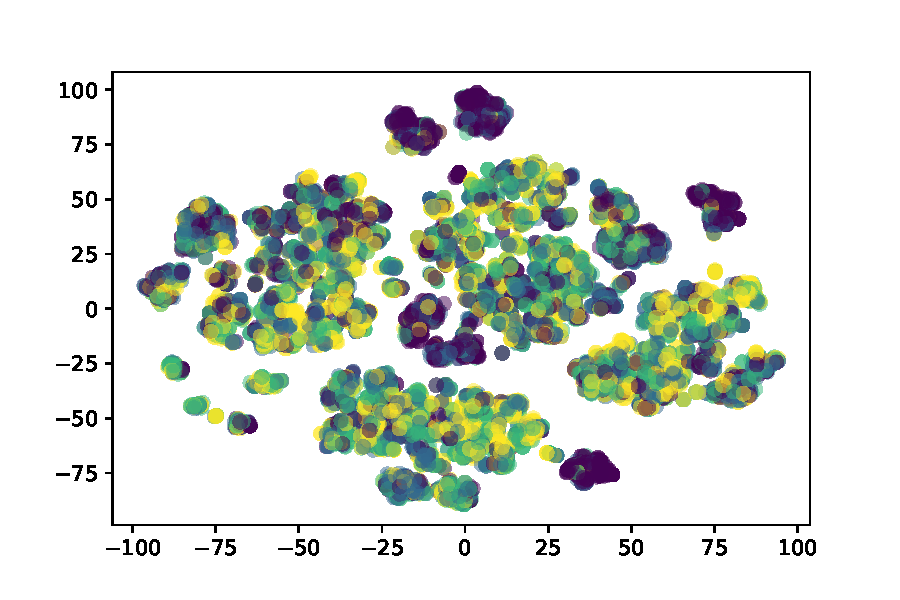
\includegraphics[width=0.4\textwidth]{img/clusters/tsne-labels.pdf}}
  \caption{Two-dimensional embeddings of the training data using the PCA and t-SNE algorithms, where color corresponds to the true price label.}
  \label{fig:cluster-labels}
\end{figure}

Both seem to show 4 potential clusters, so I ran the K-means algorithm (implementation details are in the Training section of this report) on the data with $K=4$ to divide the data into 4 parts. Figure \ref{fig:clusters} shoes the data embeddings again, but each point is colored according to its cluster assignment instead of its true price label. 
\begin{figure}[H]
  \centering
  \subfloat[PCA]{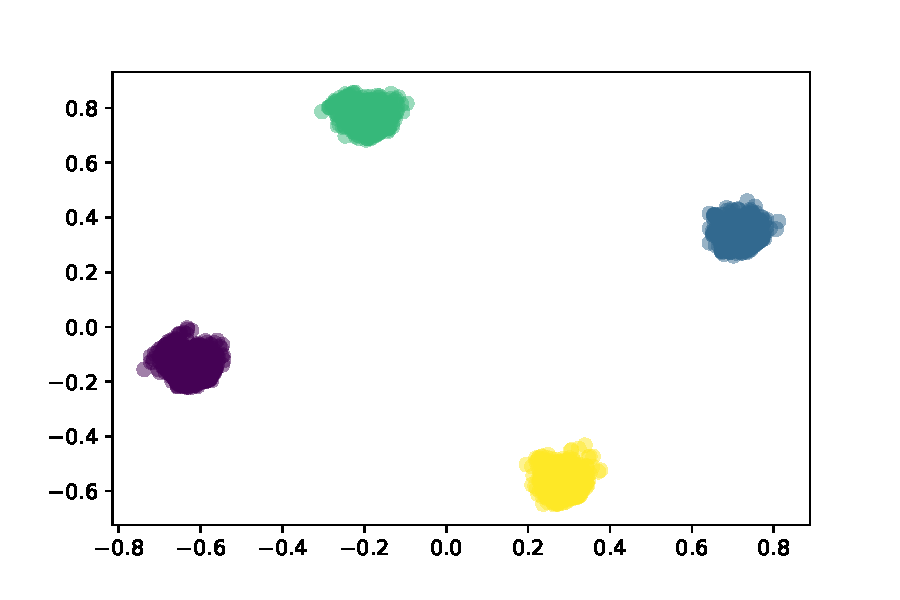
\includegraphics[width=0.4\textwidth]{img/clusters/clusters.pdf}}
  \subfloat[t-SNE]{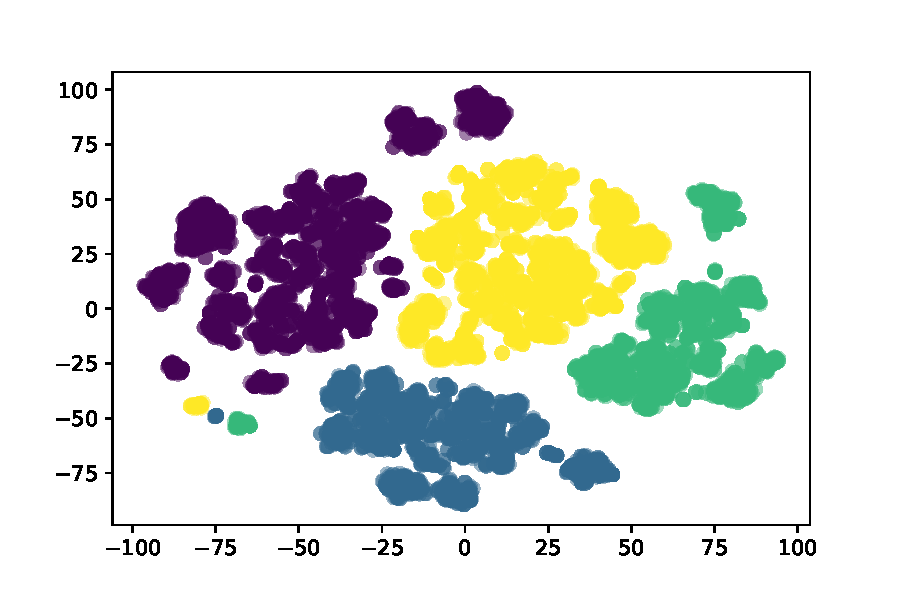
\includegraphics[width=0.4\textwidth]{img/clusters/tsne-clusters.pdf}}
  \caption{Two-dimensional embeddings of the training data using the PCA and t-SNE algorithms, where color corresponds to the assigned cluster.}
  \label{fig:clusters}
\end{figure}

This seems like a good qualitative match with the data, so I saved the cluster centers. I planned on creating 4 separate classifiers - 1 for each cluster. To make a price prediction for a single data point, I would determine its nearest cluster center, then use that cluster's classifier in order to make a prediction. My intuition here was that I could perhaps remove some of the complexity in the relationship between data and labels by manually splitting up data that was very different. This might allow each of the 4 individual models to pick up on local patterns in the data that were \textbf{not} global patterns in the data.

\subsubheader{Neighborhood Clusters}

In addition to clustering the data as a whole, I also examined the geographic locations of the neighborhoods. Figure \ref{fig:nhoods} shows the coordinates of each neighborhood, where the $x$-axis is longitude and the $y$-axis is latitude. Unlike with the data as a whole, there was no clear number of clusters for this data. To protect against overfitting, I set the number of clusters to 3, which seems to split the data without making any of the clusters too small. Similar to the training method used with the previous clustering strategy, I planned on dividing up the data based on which neighborhood cluster it belonged to, then using that to determine which of three classifiers it should use for its prediction. My intuition here was that geographically proximate neighborhoods should have similar ppopulation densities, and thus should have similar styles of housing, similar patrons, and, similar prices distributions.

\begin{figure}[H]
  \centering
  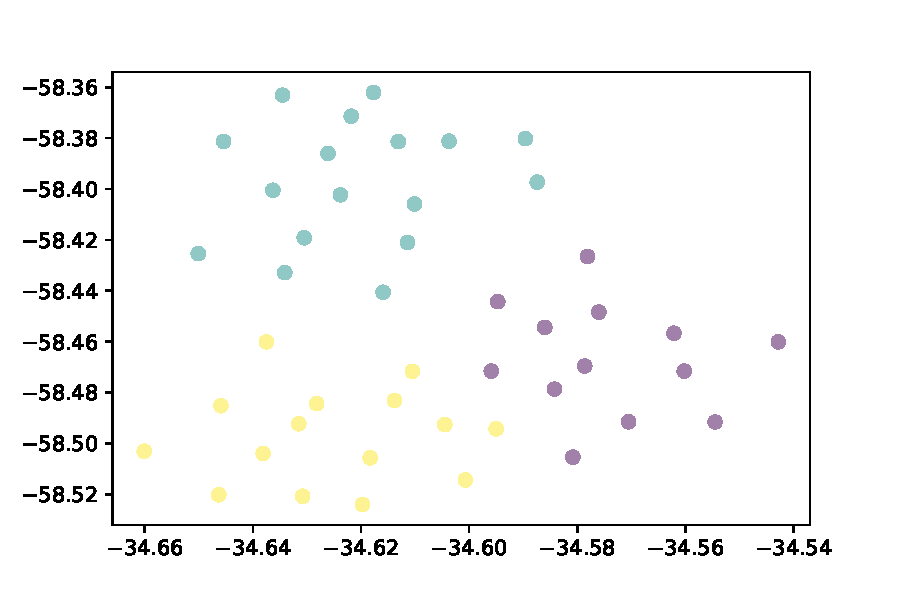
\includegraphics[width=0.45\textwidth]{img/clusters/nhoods.pdf}
  \caption{The geographic locations of the neighborhoods from the training data, split into three clusters.}
  \label{fig:nhoods}
\end{figure}

% ======
% MODELS
% ======
\subheader{Models}

With such complex data, I assumed that the relationship between the data and the labels would be non-linear. Thus, methods like SVM with RBF kernel and decision trees seemed like appealing choices. I was wary of using SVM, as I did not want to overfit to the training data, but still wanted to take advantage of their expressive power.

The two models I settled on were
\begin{enumerate}
	\item an SVM model with RBF kernel, with parameters $\gamma=0.5$ and $C=50$; and
	\item a random forest, where each individual decision tree had a maximum depth of 20.
\end{enumerate}

Although I did test standard decision trees, I used random forests for my main model instead because of their greater expressive power. Details of how I chose the aforementioned hyperparameters are in the Hyperparameter Selection section of this report.

I decided on using standard random forests instead of a cluster-based variant for my final model after significant testing. Since the cluster-based hybrid models were a significant amount of my work on this project, though, I still include details of how I trained them and selected hyperparameters later on.

Another factor in my decision to use these two families of models is the existence of easy-to-use libraries implementing both models. I used the Scikit-Learn library to create and train my models. For the SVM, I was able to use the library's `svm.SVC' model directly and only worry about changing hyperparameters. For the cluster-random forest hybrid models, I was able to create a custom Scikit-Learn classifier that managed multiple random forests at once and used pre-determined clusters to decide which classifier to use when making a prediction on a given data point. The random forests in my cluster models were implemented using the `ensemble.RandomForestClassifier' model from Scikit-Learn.\cite{scikit-learn}

Since both of my families of models were implemented in this way, I was able to use standard Scikit-Learn cross validation functions on both, which I go into more detail on in the Data Splits section of this report.


% ========
% TRAINING
% ========
\newpage
\subheader{Training}

\subsubheader{Training Algorithms}

The Scikit-Learn SVM model that I used implements multi-class classification by training 6 classifiers (the number of combinations of 2 classes when there are 4 classes total). It is able to decide what class a given point belongs to by running the two-class classifiers on each combination of classes and choosing the single class that beats out the rest.

In order to train the SVM in the first place, the library approximately solves the primal optimization problem
\[
\min_{w,b,\zeta} \frac{1}{2} w^T w + C \sum_{i=1}^{n} \zeta_i
\] such that $y_i (w^T \phi(x_i) + b) \geq 1 - \zeta_i$ and $\zeta_i \geq 0$ for all $i$. In this case, $\phi$ is a map from our given feature space to the feature space under the RBF kernel and $\zeta_i$ is the error for point $i$.

In order to solve this, the library instead solves the dual optimization problem
\[
\min_\alpha \frac{1}{2} \alpha^T Q \alpha - e^T \alpha,
\] such that $y^T \alpha = 0$ and $0 \leq \alpha_i \leq C$ for all $i$. In this formulation, $Q_{ij} = y_i y_j K(x_i, x_j)$, where $K$ is the RBF kernel.

In order to actually solve this dual problem, Scikit-Learn uses the libsvm library, which itself uses Sequential Minimal Optimization (SMO) to solve the dual.\cite{libsvm}

The Scikit-Learn RandomForestClassifier constructs decision trees based on bootstrap samples from the training data. The splits in each decision tree in the forest are allowed to choose from $\sqrt{n}$ features, where $n$ is the total number of features. The splits are chosen to maximize the Gini index.

Each decision tree outputs a probabilistic answer. If a leaf node in a decision tree has proportion $p$ of class 1 and if $p$ is the largest proportion of the classes, then the decision tree(assuming it reaches this particular leaf node) will output class 1 along with $p$. This gives each prediction a sense of certainty. When combining the predictions from each tree in the forest, the Scikit-Learn implementation combines these probabilities instead of just counting how many trees voted for which class.

\subsubheader{Runtime}

In terms of wall time, the random forest method was the fastest to train, taking approximately one minute to run through parameter sweeps on my laptop. The SVM model was slower, taking anywhere between 1 and 5 minutes, depending on how many other tasks were currently running on my computer. The cluster-based hybrid models took significantly longer, mainly due to an inefficient prediction function. They frequently took longer than 10 minutes to train when using parameter sweeps.

In order to train just a single model with no parameter sweeps, the random forest took a matter of seconds, SVM took a decent fraction of a minute, and the cluster-based model frequently took over a minute.


% ========================
% HYPERPARAMETER SELECTION
% ========================
\subheader{Hyperparameter Selection}

In order to select hyperparamters, I used a series of searches across what seemed like reasonable chunks of parameter space. For my random forest models, I only varied the maximum depth parameter. To find the optimal parameter, I fixed all others and ran $K$-fold\footnote{For the cluster-based random forest methods, I only used 3 folds because of computational constraints. For the standard random forest model, I used 10 folds.} cross validation on models with varied values of the maximum depth parameter. I selected the parameter value with the maximum validation accuracy.

\begin{figure}[H]
  \centering
  \subfloat[]{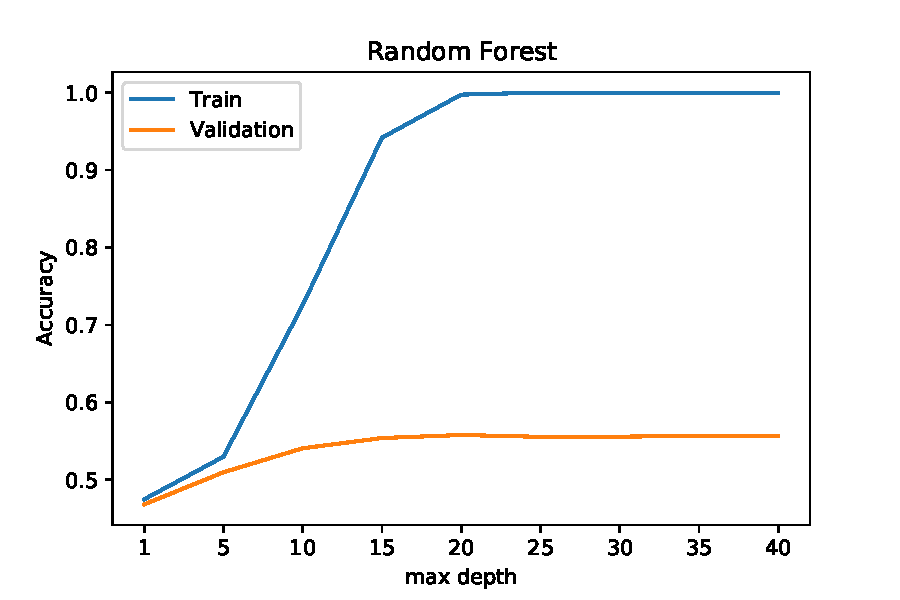
\includegraphics[width=0.3\textwidth]{img/training/rf_removed.pdf}}
  \subfloat[]{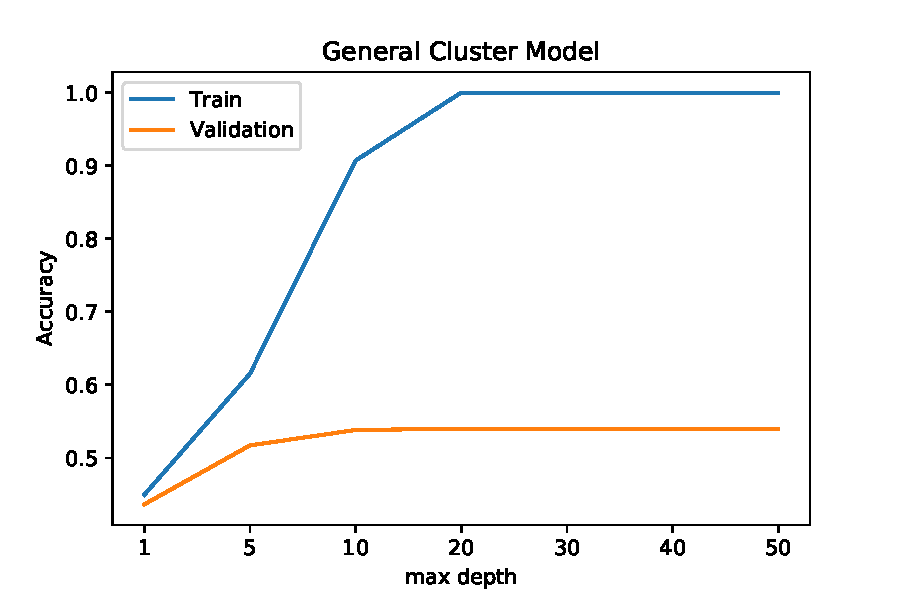
\includegraphics[width=0.3\textwidth]{img/training/hybrid_removed.pdf}}
  \subfloat[]{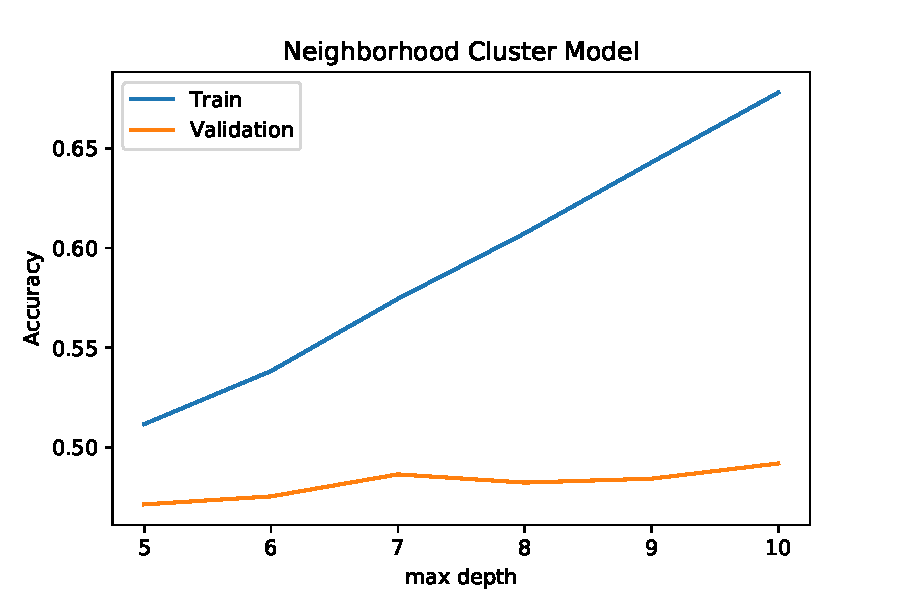
\includegraphics[width=0.3\textwidth]{img/training/nhood_removed.pdf}}
  \caption{Training and validation curves for both cluster-based hybrid models: (a) Random Forest, (b) General Cluster-based model, and (c) neighborhood cluster-based model.}
  \label{fig:training-clusters}
\end{figure}

For the SVM model, I tuned both the RBF kernel parameter $\gamma$ and the regularization coefficient $C$. Instead of just varying one of the constants, I created a grid of possible parameter values, where each square in the grid represented a different combination of parameters. I used cross validation on a model for each square in the grid, and chose the parameters from the square with the highest validation accuracy. Figure \ref{fig:svm-params} shows the training and validation accuracies from this process.

\begin{figure}[H]
  \centering
  \subfloat[Training]{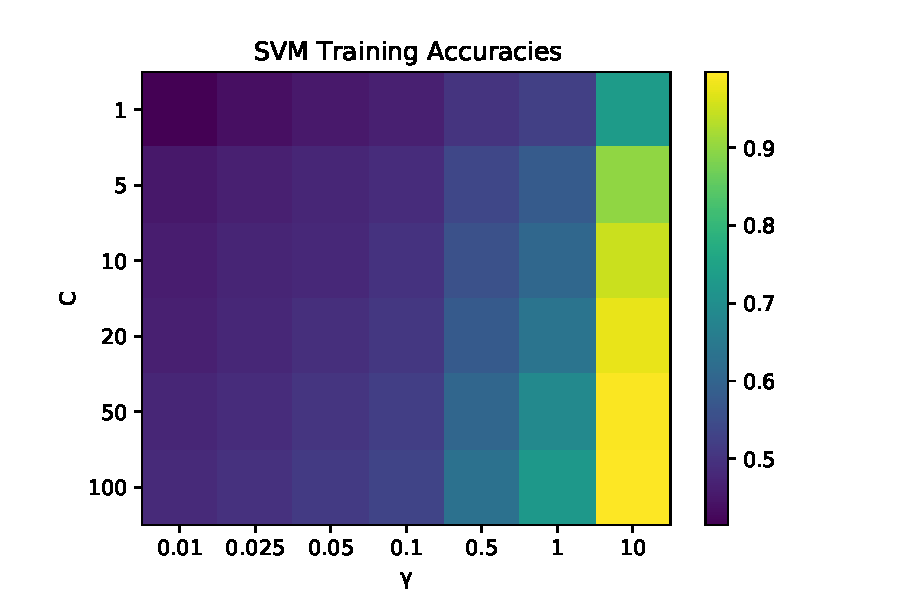
\includegraphics[width=0.4\textwidth]{img/training/svm_train_removed.pdf}}
  \subfloat[Validation]{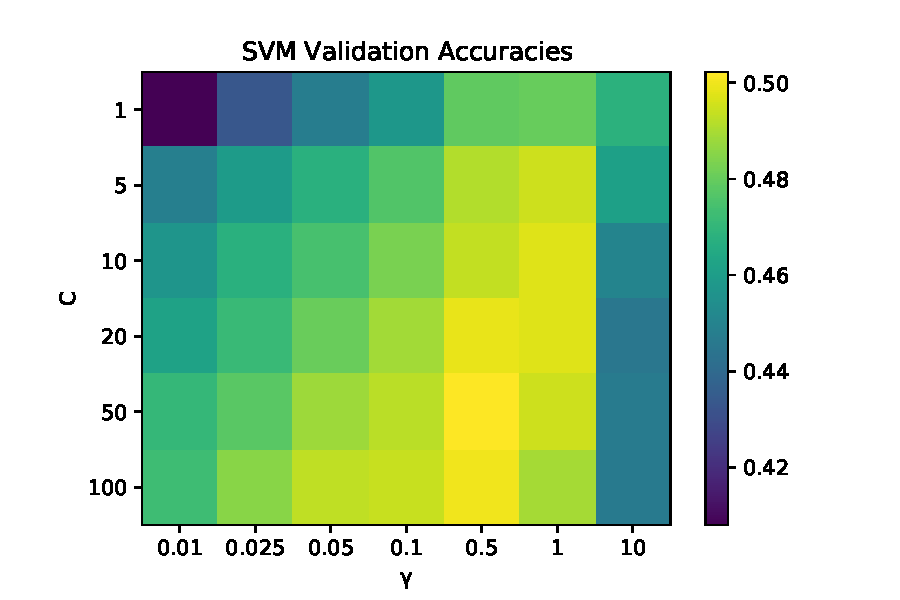
\includegraphics[width=0.4\textwidth]{img/training/svm_val_removed.pdf}}
  \caption{Training and Validation accuracies from the cross validation scheme for the SVM model.}
  \label{fig:svm-params}
\end{figure}


% ===========
% DATA SPLITS
% ===========
\subheader{Data Splits}

All of my models used the same cross validation scheme to determine model performance. I divided the training set into $K$ folds of equal size, and cycled through the folds, setting one to be the validation fold and the others to be the training folds. To evaluate a model, I trained it using the training folds and tested it using the validation fold. I repeated this for each fold cycle and averaging the training and testing accuracies to get my final performance metrics. This process was implemented using the Scikit-learn `KFold' method.

Although I kept track of the training accuracies in this process, the validation/testing accuracy was more important, as this gave me a sense of how well my models generalized to unseen data, i.e. how well they avoided overfitting.

% ===================
% ERRORS AND MISTAKES
% ===================
\newpage
\subheader{Errors and Mistakes}

Throughout my experiments, I ran into the common pitfall of not managing the variables in my Jupyter notebooks neatly enough. Every so often, I would realize that I was using a variable name that I had deleted, but my code was not failing because that particular variable still existed in my current session. This is a somewhat artificial error, but I needed to mention it nonetheless since it did delay my progress by a non-trivial amount.

The biggest mistake I made during this project was probably trying to dive right into the model development phase without spending enough time interacting with the data. Originally, I just converted all my data to floating point numbers and then began experimenting with SVM and random forest models. After about a day of this, I realized that I did not understand what my data was, and I went back to the data preparation stage. It was only then that I was able to do feature engineering and determine correlated features.

The hardest part of this project was being creative with unfamiliar data. In earlier assignments, if we needed to use data, it was straightforward and worked out-of-the-box. This time around, however, I had to manipulate and analyze the data in order to make it more informative. This was my first experience with feature engineering and in-depth data analysis, so it required a lot of experimentation on my part.

% ===================
% PREDICTIVE ACCURACY
% ===================
\subheader{Predictive Accuracy}

\textit{The results in this section correspond to the testing accuracy displayed prior to the end of the competition, which was calculated using only a portion of the full test set. My final results may be slightly different than these. For reference, my Kaggle username is bradenhoagland.}

\begin{figure}[H]
  \centering
  \subfloat[Random Forest]{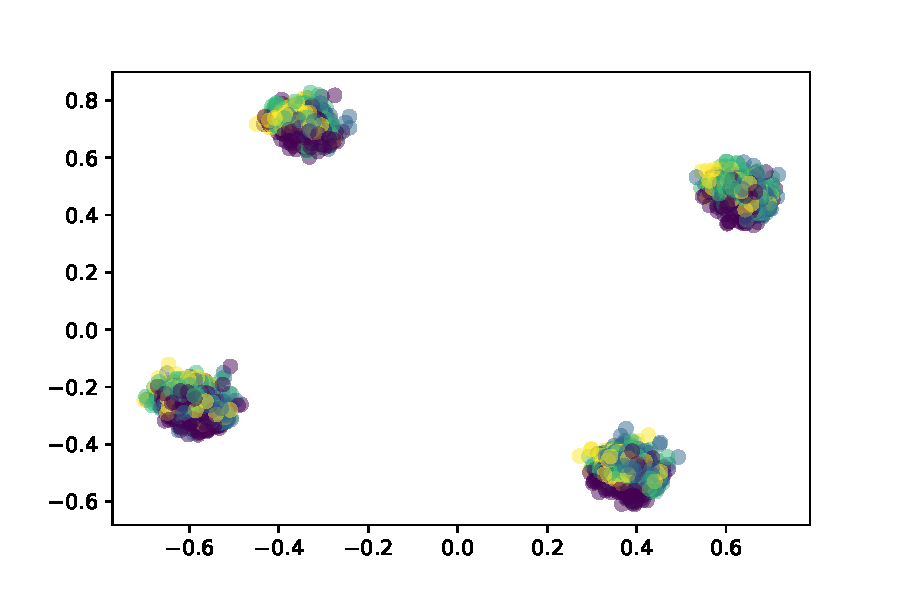
\includegraphics[width=0.4\textwidth]{img/preds/forest.pdf}}
  \subfloat[SVM]{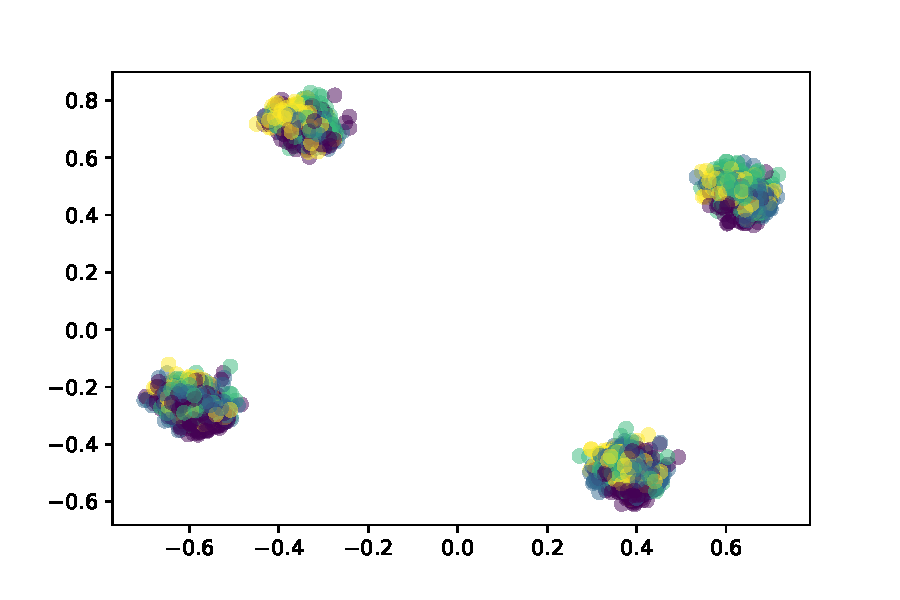
\includegraphics[width=0.4\textwidth]{img/preds/svm.pdf}}
  \caption{Model predictions on the test set. The random forest predictions shown come from the non-clustering model.}
  \label{fig:preds}
\end{figure}

My SVM model, even with correlated features removed, was only able to achieve 52\% test accuracy. Although its training accuracy was close to perfect, the expressive power of the RBF kernel was not limited enough for it to generalize well. I could have potentially improved the generalization ability of this model through more hyperparamter tuning, but the results from my hybrid models were promising enough that I focused on those instead.

Before removing correlated features, my standard random forest model was able to achieve 55\% test accuracy. After removing corrleated features, this became 56\%. Perhaps not surprisingly, adding clusters resulted in poorer generalization, with my general cluster model having 54.5\% test accuracy and my neighborhood cluster model having 49.5\% test accuracy. The general clusters gave the random forest model better training accuracy, but the neighborhood clusters resulted in both poorer trianing and poorer validation accuracy. The accuracy curves in Figure \ref{fig:training-clusters} from the Hyperparameter Selection section of this report support this claim.

Figure \ref{fig:preds} shows 2-dimensional PCA embeddings of the test set, where the points are colored based on the class prediction of the respective model. Both models can be seen to be very similar, with only slight differences in some areas of each cluster.

% ====
% CODE
% ====
\subheader{Code}

Below are the two Jupyter notebooks I used for this project. Almost all the outputs should be there, with the one major exception of the density plots that I used during my exploratory data analysis. They took up almost 10 pages on their own, so I removed them from the output.

The first PDF is my main training notebook, which has almost all of the results. The second PDF is the notebook I used to train my neighborhood cluster-based model. The training pipeline for this model was different, thus a second notebook. As a result, much of the code in the second notebook can also be found in the first notebook.

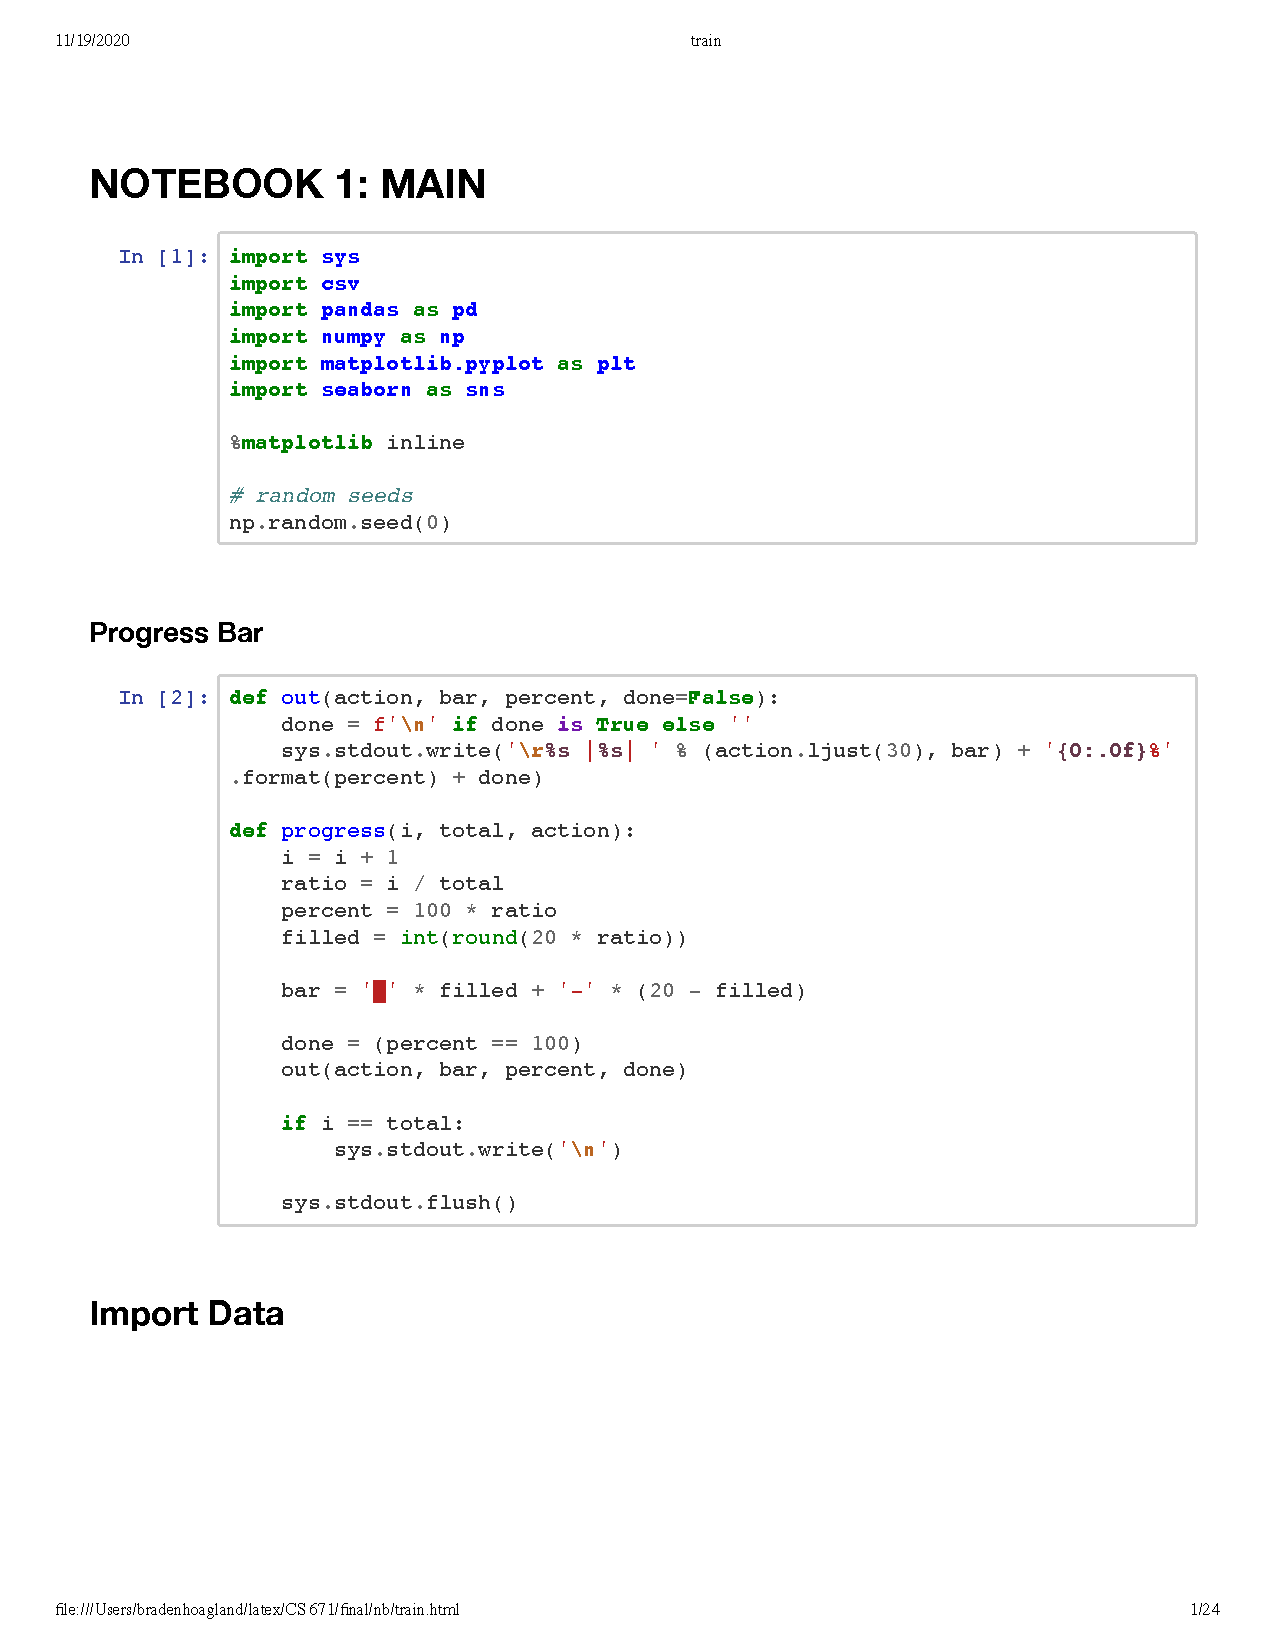
\includepdf[pages=-, width=\textwidth]{nb/train.pdf}

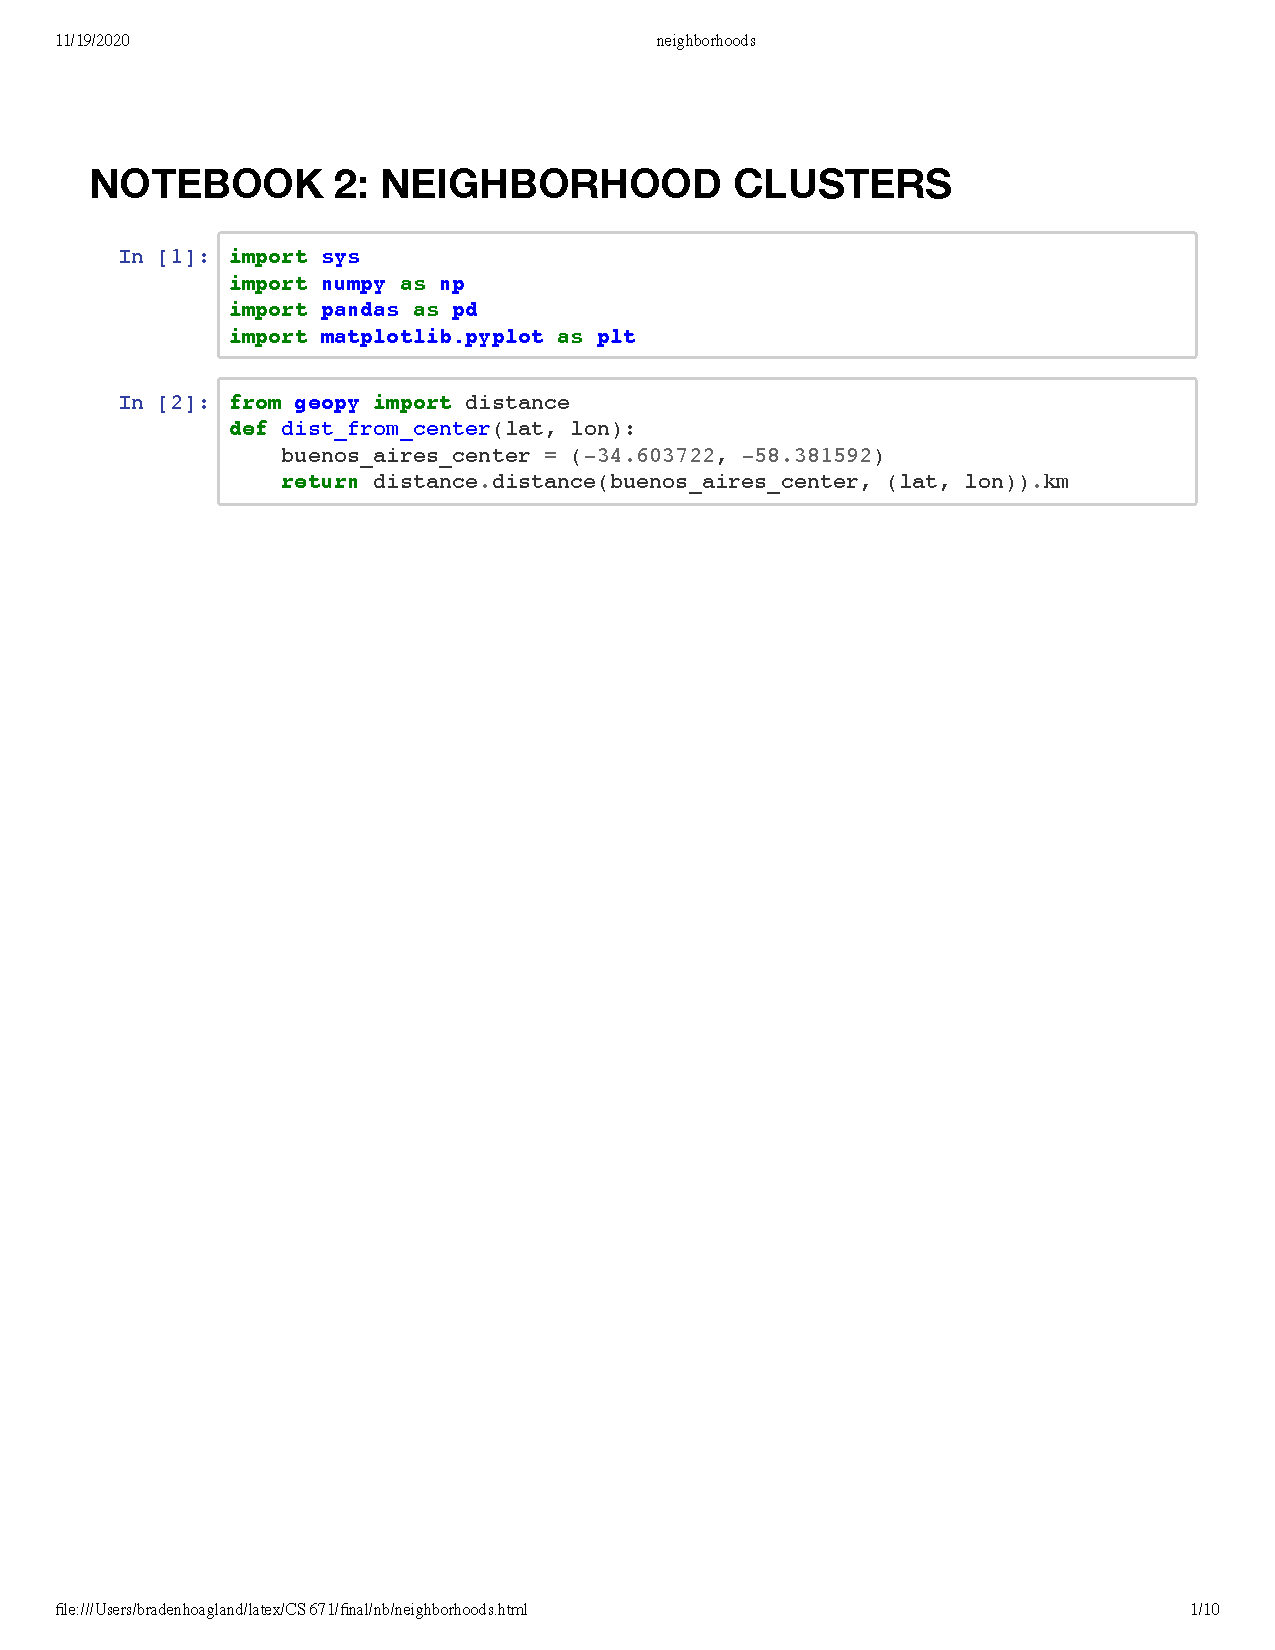
\includepdf[pages=-, width=\textwidth]{nb/neighborhoods.pdf}


% \newpage
\subheader{References}

\bibliography{final}
\bibliographystyle{plain}

\end{document}

